%------------------------------------------%
% Cannabis Data Science
% Saturday Morning Statistics
% Date: 3/19/2022
%------------------------------------------%
\documentclass[xcolor={dvipsnames}]{beamer}
\hypersetup{pdfpagemode = FullScreen}
\mode<presentation>{
  \usetheme{Boadilla}
  \usecolortheme{orchid}
  \usefonttheme{default}
  \setbeamertemplate{navigation symbols}{}
  \setbeamertemplate{caption}[numbered]
}
\setbeamersize{
  text margin left = 0.5in,
  text margin right = 0.5in
}

%------------------------------------------%
% Title
%------------------------------------------%
\author{Cannabis Data Science}
\title[\textbf{Saturday Morning Statistics \#16}]{}
\institute[]{\Large Saturday Morning Statistics \#16}
\date{March \nth{19}, 2022}

%------------------------------------------%
% Packages
%------------------------------------------%
\usepackage[english]{babel}
\usepackage[utf8x]{inputenc}
\usepackage{tikz}
\usepackage{xparse}

%------------------------------------------%
% Colors
%------------------------------------------%
\definecolor{Green}{RGB}{34, 153, 84}
\definecolor{LightGreen}{RGB}{218, 247, 166}
\definecolor{DarkGreen}{RGB}{2, 48, 32}
\definecolor{Orange}{RGB}{255, 87, 51}
\definecolor{DarkOrange}{RGB}{199, 0, 57}
\definecolor{Yellow}{RGB}{255, 195, 0}

%------------------------------------------%
% Theme
%------------------------------------------%
\setbeamercolor*{palette primary}{bg=LightGreen, fg=DarkGreen}
\setbeamercolor*{palette secondary}{bg=LightGreen, fg=DarkGreen}
\setbeamercolor*{palette tertiary}{bg=LightGreen, fg=DarkGreen}

%------------------------------------------%
% Packages
%------------------------------------------%
\usepackage{amsmath}
\renewcommand*\footnoterule{} % No separating line on footnote.
\usepackage{mathtools} % For annotating equations.
\usepackage{hhline} % for double bars.
\usepackage[super]{nth} % For formatting 1st, 2nd, 3rd, etc.
\usepackage{graphicx, caption, subcaption}
\usepackage{setspace}
%\usepackage{enumitem}

%------------------------------------------%
% Commands
%------------------------------------------%

% Top space.
\newcommand\T{\rule{0pt}{2.5ex}}

% Bottom space.
\newcommand\B{\rule[-1.25ex]{0pt}{0pt}}

% Blocks.
\newenvironment<>{Block}[2][.9\textwidth]
  {\setlength{\textwidth}{#1}
  \begin{actionenv}#3
    \def\insertblocktitle{#2}\par
    \usebeamertemplate{block begin}}
  {\par\usebeamertemplate{block end}
  \end{actionenv}}

% Balls.
\defbeamertemplate{enumerate item}{largeball}
{\begin{pgfpicture}{-1ex}{-0.65ex}{1.5ex}{1.5ex}
\usebeamercolor[fg]{item projected}
{\pgftransformscale{2.5}\pgftext{\Large\pgfuseshading{bigsphere}}}
{\pgftransformshift{\pgfpoint{0pt}{0.5pt}}
\pgftext{\usebeamerfont*{item projected}\small\insertenumlabel}}
\end{pgfpicture}}

% Fancy arrows.
\NewDocumentCommand\UpArrow{O{2.0ex} O{black}}{%
   \mathrel{\tikz[baseline] \draw [->, line width=0.5pt, #2] (0,0) -- ++(0,#1);}} % Fancy up-arrow.
\NewDocumentCommand\DownArrow{O{2.0ex} O{black}}{%
   \mathrel{\tikz[baseline] \draw [<-, line width=0.5pt, #2] (0,0) -- ++(0,#1);}} % Fancy down-arrow.

% Equations with numbers on the left.
\makeatletter
\newcommand{\LeftEqNo}{\let\veqno\@@leqno}
\makeatother

%------------------------------------------%
% Presentation
%------------------------------------------%
\begin{document}

%------------------------------------------%
% Title Page
%------------------------------------------%
\begin{frame}{}
  
\includegraphics[scale=0.33]{images/logo.pdf}
  \vspace*{-2\baselineskip}
  \titlepage
\end{frame}

%------------------------------------------%
% Data Science
%------------------------------------------%

\begin{frame}{The State of Data Science}

\begin{minipage}{0.6\textwidth}

\vspace{-1\baselineskip}

\small

Avenues for advancing {\bfseries data tidying}:

\vspace{0.5\baselineskip}
\begin{itemize}

\setlength{\parindent}{0pt}

\item Correcting character encodings; 
\includegraphics[height=.175in]{images/check.png}

\vspace{0.25\baselineskip}

\item Parsing dates and numbers; 
\includegraphics[height=.175in]{images/check.png}

\vspace{0.25\baselineskip}

\item Identifying missing values; 
\includegraphics[height=.175in]{images/check.png}

\vspace{0.25\baselineskip}

\item {\color{Green} Matching similar but not identical values};

\vspace{0.25\baselineskip}

\item {\color{Green} Filling in structural missing values};

\vspace{0.25\baselineskip}

\item {\color{Green} Model-based data cleaning}.

\end{itemize}

\end{minipage}\hspace{0.05\textwidth}%
\begin{minipage}{0.345\textwidth}

\begin{figure}
\includegraphics[width=\textwidth]{images/melting-data.png}
\caption*{\small Melting data.}
\end{figure}

\begin{figure}
\includegraphics[width=\textwidth]{images/pairing-data.png}
\caption*{\small Pairing data.}
\end{figure}

\end{minipage}

\vspace{0.5\baselineskip}

{\scriptsize Reference: Tidy Data, Hadley Wickham, Journal of Statistical Software (2014).}

\end{frame}

%------------------------------------------%
% Statistical History
%------------------------------------------%

% Optional: Add a bit of statistical history.

\begin{frame}{A Peek at Scientific History}

\small

\vspace{0.25\baselineskip}

{\textbf{Taxonomy}} is the scientific study of \underline{naming}, \underline{defining}, and \underline{classifying} groups of biological organisms based on shared characteristics.

\vspace{0.75\baselineskip}

\begin{minipage}{0.65\textwidth}

Taxonomic characteristics used to differentiate {\bfseries taxa} include:

\vspace{0.25\baselineskip}
\begin{itemize}

\item Morphological;

\vspace{0.125\baselineskip}

\item Physiological;

\vspace{0.125\baselineskip}

\item Molecular;

\vspace{0.125\baselineskip}

\item Behavioral;

\vspace{0.125\baselineskip}

\item Ecological;

\vspace{0.125\baselineskip}

\item Geographic.

\end{itemize}

\vspace{0.5\baselineskip}

A {\bfseries strain} is a genetic variant, a subtype or a culture within a biological species.

\end{minipage}\hspace{0.05\textwidth}%
\begin{minipage}{0.25\textwidth}

\begin{figure}
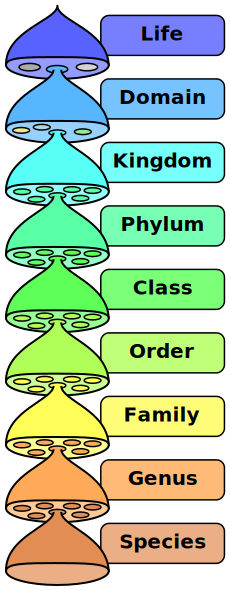
\includegraphics[width=\textwidth]{images/biological-classification.png}
\end{figure}

\end{minipage}

\end{frame}


%------------------------------------------%
% Application to cannabis research
%------------------------------------------%

\begin{frame}{Application to cannabis research}

\vspace{0.5\baselineskip}
{\large \textbf{The Indica / Sativa Dichotomy}}\\[0.5\baselineskip]

\begin{minipage}{0.25\textwidth}

\begin{figure}
\includegraphics[width=0.8\textwidth]{images/lamarck.jpg}
\end{figure}

\end{minipage}\hspace{0.05\textwidth}%
\begin{minipage}{0.7\textwidth}

\footnotesize
Jean-Baptiste de {\bfseries Lamarck} (1744 - 1829)\\
Notable naturalist, biologist, and taxonomer.\\Collector of rare plants.

\begin{itemize}

\item Named {\itshape Cannabis indica} (the \nth{2} cannabis species).

\begin{itemize}

\footnotesize

\item Hindu Kush mountain range;

\item Temperate climates;

\item The {\itshape \color{Green} botanical defence} (1970s).

%\item The name, {\itshape Cannabis sativa}, was found to be in the domain of judicial, not scientific, authority.  

\end{itemize}

\end{itemize}

\end{minipage}

\vspace{0.5\baselineskip}

\begin{minipage}{0.55\textwidth}

\footnotesize

\vspace{-1.5\baselineskip}
\begin{itemize}

\item {\bfseries Claim:} {\itshape Cannabis indica} strains tend to have higher {\color{Red}THC} content than {\itshape Cannabis sativa} strains (Fischedick et. al 2010, Hillig and Mahlberg 2004).

\vspace{0.5\baselineskip}

\item {\bfseries Claim:} Known indica strains include {\itshape\color{OliveGreen} Kush}, {\itshape\color{Aquamarine} Northern Lights}, and {\itshape\color{Purple} Purple Kush}.

\end{itemize}

\end{minipage}\hspace{0.05\textwidth}%
\begin{minipage}{0.4\textwidth}

\begin{figure}
\includegraphics[height=0.95in]{images/plants.jpg}
\caption*{
\tiny New born Cannabis plants (2017).\\
{\tiny\color{Gray}
Author: Mar11, 
License: CC BY-SA 4.0 \\https://creativecommons.org/licenses/by-sa/4.0}
}
\end{figure}

\end{minipage}

\end{frame}


%------------------------------------------%
% Question and Hypothesis
%------------------------------------------%
\section{Introduction}
\begin{frame}{Question and Hypothesis}

% Question of the day
\begin{center}
\begin{minipage}{.9\linewidth}
\begin{Block}{Question of the day.}

\vspace{.5\baselineskip}
\begin{itemize}

\item Can we build a model to predict a cannabis product's {\bfseries strain} given a readily available factors, such as:

\vspace{.25\baselineskip}
\begin{itemize}

\item If the product is a {\itshape\color{OliveGreen} Kush}.

\vspace{.5\baselineskip}

\item If the product is {\color{Purple}purple}.

\vspace{.5\baselineskip}

\item The {\color{Red}THC} concentration of the product, perhaps relative to the {\color{Brown}CBD} concentration.

\end{itemize}

\end{itemize}

\vspace{.5\baselineskip}

\end{Block}
\end{minipage}
\end{center}

\end{frame}


%------------------------------------------%
% Methodology: Probit Models
%------------------------------------------%

\begin{frame}{Methodology: Probit Models}

Given a latent variable representation of the {\bfseries probit model}:

\begin{align*}
z_i &= x_i\beta + \epsilon _i, \hspace{4ex} \epsilon _i \stackrel{iid}{\sim} \mathcal{N}(0, 1), \\
\\[-0.5\baselineskip]
y_i &=
  \begin{cases}
    1 \text{ if } z_i > 0\\
    0 \text{ if } z_i \leq 0
  \end{cases}
\end{align*}

\vspace{0.5\baselineskip}
You can estimate the parameters using the {\bfseries likelihood function}

$$
L(\beta) = \prod_{i=1}^n\Phi(x_i\beta)^{y_i}[1 - \Phi(x_i\beta)]^{1-y_i}.
$$

\end{frame}


%------------------------------------------%
% Takeaway
%------------------------------------------%
\section{Takeaway}
\begin{frame}{}

\begin{center}
\begin{minipage}{3.85in}

% Thank you.
\begin{center}
\includegraphics[width=.25in]{images/prayer.png} {\Large \textbf{Thank you for coming.}}\\
\end{center}
\vspace*{0.5\baselineskip}

% Re-cap the lesson of the week.
\begin{center}
\begin{minipage}{\linewidth}
\begin{Block}{Lesson of the Day}

\vspace{0.5\baselineskip}

\begin{itemize}

\item Names are powerful.

\vspace{0.5\baselineskip}

\end{itemize}

\end{Block}
\end{minipage}
\end{center}

\vspace*{2\baselineskip}

\end{minipage}
\end{center}

\end{frame}


%------------------------------------------%
% Fin.
%------------------------------------------%
\end{document}
